% ============================================================
%  ОТЧЁТ
%  Лабораторная работа №2
%  Дисциплина: Информационно-поисковые системы
%  РУДН, 2025
% ============================================================

\documentclass[12pt, a4paper]{report}

% ── Кодировки и язык ────────────────────────────────────────
\usepackage[utf8]{inputenc}
\usepackage[T2A]{fontenc}
\usepackage[russian, english]{babel}

% ── Геометрия страницы (ГОСТ 7.32) ──────────────────────────
\usepackage[
  left   = 30mm,
  right  = 15mm,
  top    = 20mm,
  bottom = 20mm
]{geometry}

% ── Шрифты ──────────────────────────────────────────────────
\usepackage{mathptmx}          % Times New Roman (основной текст)
\usepackage{helvet}            % Helvetica (заголовки)
\usepackage[scaled=0.85]{beramono} % моноширинный шрифт
\usepackage{amsfonts}

% ── Межстрочный интервал и отступы ──────────────────────────
\usepackage{setspace}
\setstretch{1.5}               % полуторный интервал (ГОСТ)

\usepackage{indentfirst}
\setlength{\parindent}{1.25cm}
\setlength{\parskip}{0pt}

% ── Заголовки разделов ───────────────────────────────────────
\usepackage{titlesec}

\titleformat{\chapter}[block]
  {\sffamily\Large\bfseries\color{NavyBlue}}
  {\thechapter.}{0.5em}{}
\titlespacing{\chapter}{0pt}{12pt}{8pt}

\titleformat{\section}[block]
  {\sffamily\large\bfseries\color{SteelBlue}}
  {\thesection.}{0.5em}{}
\titlespacing{\section}{0pt}{10pt}{6pt}

\titleformat{\subsection}[block]
  {\sffamily\normalsize\bfseries\color{SteelBlue!80!black}}
  {\thesubsection.}{0.5em}{}
\titlespacing{\subsection}{0pt}{8pt}{4pt}

% ── Цвета ────────────────────────────────────────────────────
\usepackage[dvipsnames, table]{xcolor}
\definecolor{NavyBlue}   {RGB}{31,  78, 121}
\definecolor{SteelBlue}  {RGB}{46, 117, 182}
\definecolor{LightBlue}  {RGB}{222,234,246}
\definecolor{PlaceholderBg}{RGB}{255,251,230}
\definecolor{PlaceholderBorder}{RGB}{200,180,120}
\definecolor{CodeBg}     {RGB}{245,245,245}
\definecolor{CodeBorder} {RGB}{46, 117, 182}

% ── Таблицы ─────────────────────────────────────────────────
\usepackage{booktabs}
\usepackage{tabularx}
\usepackage{multirow}
\usepackage{longtable}
\usepackage{array}
\renewcommand{\arraystretch}{1.4}

% ── Листинги кода ────────────────────────────────────────────
\usepackage{listings}
\lstset{
  language        = Python,
  basicstyle      = \ttfamily\small,
  keywordstyle    = \bfseries\color{NavyBlue},
  commentstyle    = \itshape\color{gray},
  stringstyle     = \color{SteelBlue!80!black},
  backgroundcolor = \color{CodeBg},
  frame           = leftline,
  framerule       = 2pt,
  rulecolor       = \color{CodeBorder},
  numbers         = left,
  numberstyle     = \tiny\color{gray},
  numbersep       = 8pt,
  showstringspaces= false,
  breaklines      = true,
  breakatwhitespace= true,
  inputencoding   = utf8,
  extendedchars   = true,
  literate        = % поддержка кириллицы в lstlisting
    {а}{{\cyra}}1 {б}{{\cyrb}}1 {в}{{\cyrv}}1 {г}{{\cyrg}}1
    {д}{{\cyrd}}1 {е}{{\cyre}}1 {ж}{{\cyrzh}}1 {з}{{\cyrz}}1
    {и}{{\cyri}}1 {й}{{\cyrishrt}}1 {к}{{\cyrk}}1 {л}{{\cyrl}}1
    {м}{{\cyrm}}1 {н}{{\cyrn}}1 {о}{{\cyro}}1 {п}{{\cyrp}}1
    {р}{{\cyrr}}1 {с}{{\cyrs}}1 {т}{{\cyrt}}1 {у}{{\cyru}}1
    {ф}{{\cyrf}}1 {х}{{\cyrh}}1 {ц}{{\cyrc}}1 {ч}{{\cyrch}}1
    {ш}{{\cyrsh}}1 {щ}{{\cyrshch}}1 {ъ}{{\cyrhrdsn}}1 {ы}{{\cyrery}}1
    {ь}{{\cyrsftsn}}1 {э}{{\cyrerev}}1 {ю}{{\cyryu}}1 {я}{{\cyrya}}1
    {А}{{\CYRA}}1 {Б}{{\CYRB}}1 {В}{{\CYRV}}1 {Г}{{\CYRG}}1
    {Д}{{\CYRD}}1 {Е}{{\CYRE}}1 {Ж}{{\CYRZH}}1 {З}{{\CYRZ}}1
    {И}{{\CYRI}}1 {К}{{\CYRK}}1 {Л}{{\CYRL}}1 {М}{{\CYRM}}1
    {Н}{{\CYRN}}1 {О}{{\CYRO}}1 {П}{{\CYRP}}1 {Р}{{\CYRR}}1
    {С}{{\CYRS}}1 {Т}{{\CYRT}}1 {У}{{\CYRU}}1 {Ф}{{\CYRF}}1
    {Х}{{\CYRH}}1 {Ц}{{\CYRC}}1 {Ч}{{\CYRCH}}1 {Ш}{{\CYRSH}}1
    {Щ}{{\CYRSHCH}}1 {Ъ}{{\CYRHRDSN}}1 {Ы}{{\CYRERY}}1 {Ь}{{\CYRSFTSN}}1
    {Э}{{\CYREREV}}1 {Ю}{{\CYRYU}}1 {Я}{{\CYRYA}}1,
  captionpos      = b,
  xleftmargin     = 1.25cm,
}

% ── Рамки и боксы ────────────────────────────────────────────
\usepackage{tcolorbox}
\tcbuselibrary{skins, breakable}

\newcommand{\placeholder}[2][Вставьте результат]{%
  \begin{tcolorbox}[colback=PlaceholderBg, colframe=PlaceholderBorder,
    fonttitle=\sffamily\small\bfseries, fontupper=\itshape\small\color{gray!60!black},
    boxrule=0.6pt, left=6pt, right=6pt, top=4pt, bottom=4pt, breakable,
    title={#2}]
    #1
  \end{tcolorbox}%
  \vspace{4pt}%
}

% ── Прочие пакеты ────────────────────────────────────────────
\usepackage{graphicx}
\usepackage{subcaption}
\usepackage{caption}
\captionsetup{font=small, labelfont={bf,sf}, labelsep=period}

\usepackage{enumitem}
\setlist[enumerate]{leftmargin=1.5cm, itemsep=2pt, parsep=0pt}
\setlist[itemize]  {leftmargin=1.5cm, itemsep=2pt, parsep=0pt}

\usepackage{hyperref}
\hypersetup{
  colorlinks = true,
  linkcolor  = NavyBlue,
  urlcolor   = SteelBlue,
  citecolor  = NavyBlue,
  pdftitle   = {Отчёт ЛР №2 — Информационно-поисковые системы},
}

\usepackage{fancyhdr}
\usepackage{lastpage}
\usepackage{amsmath}
\usepackage{microtype}

% ── Колонтитулы ──────────────────────────────────────────────
\pagestyle{fancy}
\fancyhf{}
\fancyhead[R]{\sffamily\footnotesize\color{gray}Лабораторная работа №2\ |\ Информационно-поисковые системы}
\fancyfoot[C]{\sffamily\footnotesize\color{gray}\thepage\ из\ \pageref{LastPage}}
\renewcommand{\headrulewidth}{0.4pt}
\renewcommand{\footrulewidth}{0.4pt}
\renewcommand{\headrule}{\color{SteelBlue}\hrule width\headwidth height\headrulewidth}
\renewcommand{\footrule}{\color{SteelBlue}\hrule width\headwidth height\footrulewidth}

% ── Подавление колонтитулов на chapter-страницах ─────────────
\fancypagestyle{plain}{%
  \fancyhf{}
  \fancyfoot[C]{\sffamily\footnotesize\color{gray}\thepage\ из\ \pageref{LastPage}}
  \renewcommand{\headrulewidth}{0pt}
  \renewcommand{\footrulewidth}{0.4pt}
  \renewcommand{\footrule}{\color{SteelBlue}\hrule width\headwidth height\footrulewidth}
}

% ── Нумерация глав без слова «Глава» ─────────────────────────
\renewcommand{\chaptername}{}

% ============================================================
\begin{document}
\setcounter{chapter}{0}

% ── Титульная страница ────────────────────────────────────────
\begin{titlepage}
\thispagestyle{empty}
\begin{center}

  {\sffamily\small\bfseries МИНИСТЕРСТВО НАУКИ И ВЫСШЕГО ОБРАЗОВАНИЯ\\
  РОССИЙСКОЙ ФЕДЕРАЦИИ}

  \vspace{6pt}
  {\sffamily\small\bfseries ФЕДЕРАЛЬНОЕ ГОСУДАРСТВЕННОЕ АВТОНОМНОЕ\\
  ОБРАЗОВАТЕЛЬНОЕ УЧРЕЖДЕНИЕ ВЫСШЕГО ОБРАЗОВАНИЯ}

  \vspace{8pt}
  {\sffamily\normalsize\bfseries
  <<МОСКОВСКИЙ ГОСУДАРСТВЕННЫЙ ТЕХНИЧЕСКИЙ УНИВЕРСИТЕТ ИМЕНИ Н.Э.~БАУМАНА (НАЦИОНАЛЬНЫЙ ИССЛЕДОВАТЕЛЬСКИЙ УНИВЕРСИТЕТ)>>}

  \vspace{6pt}
  {\sffamily\small Факультет \underline{Информатика и системы управления}}\\[2pt]
  {\sffamily\small Кафедра \underline{Программное обеспечение ЭВМ и информационные технологии}}

  \vspace{10pt}
  \textcolor{SteelBlue}{\rule{\linewidth}{1pt}}
  \vspace{12pt}

  {\sffamily\Large\bfseries\color{NavyBlue}
  ИНФОРМАЦИОННО-ПОИСКОВЫЕ СИСТЕМЫ}

  \vspace{20pt}

  {\sffamily\LARGE\bfseries ОТЧЁТ}\\[6pt]
  {\sffamily\large по лабораторной работе №2}

  \vspace{12pt}
  \begin{tcolorbox}[colback=LightBlue!50, colframe=NavyBlue,
    fonttitle=\sffamily\small\bfseries\color{NavyBlue}, boxrule=1pt,
    left=8pt, right=8pt, top=6pt, bottom=6pt, title={}]
    \centering\sffamily\large\bfseries\color{NavyBlue}
    Методы машинного обучения и обработки\\
    естественного языка для анализа юридических текстов
  \end{tcolorbox}

  \vspace{20pt}

  % Блок варианта
  \begin{tcolorbox}[colback=LightBlue!50, colframe=SteelBlue,
    fonttitle=\sffamily\small\bfseries\color{NavyBlue}, boxrule=1pt,
    left=8pt, right=8pt, top=6pt, bottom=6pt, title={Параметры варианта}]
    \begin{tabular}{p{5cm}p{7cm}}
      {\sffamily\small\bfseries Номер варианта}   & \underline{34\hspace{5cm}} \\[4pt]
      {\sffamily\small\bfseries Тип корпуса}      & \underline{D (Арбитражные)\hspace{2cm}} \\[4pt]
      {\sffamily\small\bfseries Метод признаков}  & \underline{TF-IDF, bigrams\hspace{2.2cm}} \\[4pt]
      {\sffamily\small\bfseries Классификатор}    & \underline{MultinomialNB\hspace{2.5cm}} \\[4pt]
      {\sffamily\small\bfseries Доп. задание}     & \underline{Anomaly Detection\hspace{1.5cm}} \\
    \end{tabular}
  \end{tcolorbox}

  \vspace{14pt}

\end{center}

% Таблица данных студента
\begin{flushright}
\begin{tabular}{p{5cm}p{7cm}}
	\toprule
	\rowcolor{LightBlue}
	\sffamily\small\bfseries Поле & \sffamily\small\bfseries Значение \\
	\midrule
	\sffamily\small Студент       & \underline{Сапожков~А.М.\hspace{3.5cm}} \\[4pt]
	\sffamily\small Группа        & \underline{ИУ7-43М\hspace{4.5cm}} \\[4pt]
	\sffamily\small Специальность & \underline{Программная инженерия\hspace{1.5cm}} \\[4pt]
	\sffamily\small Преподаватель & \underline{Курашкин~С.О.\hspace{3.5cm}} \\[4pt]
	\sffamily\small Дата сдачи    & \underline{14.03.2026\hspace{4.5cm}} \\[4pt]
	\sffamily\small Оценка        & \underline{\hspace{6.5cm}} \\
	\bottomrule
\end{tabular}
\end{flushright}

\vfill
\begin{center}
  {\sffamily\normalsize Москва, 2026}
\end{center}
\end{titlepage}

% ── Оглавление ───────────────────────────────────────────────
\tableofcontents
\thispagestyle{plain}
\clearpage

% ============================================================
%  РАЗДЕЛ 1. ЦЕЛЬ И ЗАДАЧИ
% ============================================================
\chapter{Цель и задачи работы}

Целью настоящей лабораторной работы является формирование практических компетенций
в области применения методов машинного обучения и обработки естественного языка (NLP)
к задачам автоматизированной обработки юридических текстов.

В ходе выполнения работы студент решает следующие задачи:

\begin{enumerate}
  \item Формирование и разведочный анализ тематического корпуса судебных документов
        согласно индивидуальному варианту.
  \item Реализация конвейера предобработки текстов с лемматизацией и фильтрацией стоп-слов.
  \item Извлечение числового векторного представления документов методом, предусмотренным вариантом
        (BoW, TF-IDF или символьные $n$-граммы).
  \item Обучение, настройка и сравнительная оценка алгоритмов классификации с применением
        стратифицированной кросс-валидации.
  \item Выполнение специализированного аналитического задания согласно варианту
        (обнаружение аномалий, тематическое моделирование LDA, семантический поиск,
        визуализация t-SNE, подбор гиперпараметров или нейросетевая классификация~MLP).
\end{enumerate}

% ============================================================
%  РАЗДЕЛ 2. ТЕОРЕТИЧЕСКАЯ СПРАВКА
% ============================================================
\chapter{Краткая теоретическая справка}

\begin{tcolorbox}[colback=LightBlue!50, colframe=NavyBlue,
  fonttitle=\sffamily\small\bfseries\color{NavyBlue}, boxrule=1pt,
  left=8pt, right=8pt, top=6pt, bottom=6pt, title={Источники}]
  Подробное изложение теоретического материала представлено в конспектах Лекции~3
  («Методы векторного представления текста»), Лекции~4
  («Алгоритмы классификации текстовых данных») и Лекции~5
  («Специализированные методы анализа юридических корпусов»).
\end{tcolorbox}

\vspace{8pt}

\section{Конвейер обработки текстовых данных}

Анализ юридических текстов методами машинного обучения реализуется в форме
последовательного конвейера преобразований. Каждый документ $d_i$ из коллекции
$\mathcal{D} = \{d_1, \ldots, d_N\}$ проходит через функцию предобработки
$g: D \to D'$, функцию извлечения признаков $\phi: D' \to \mathbb{R}^m$
и классификатор $f_\theta: \mathbb{R}^m \to \mathcal{Y}$.
Итоговый результат для документа $d_i$: $\hat{y}_i = f_\theta(\phi(g(d_i)))$.

\section{Методы векторного представления текста}

\textbf{Модель «мешок слов» (Bag of Words, BoW)} представляет документ вектором
абсолютных частот термов $\phi_{\text{BoW}}(d) \in \mathbb{Z}^{|V|}$, где $|V|$ —
размер словаря.

\textbf{TF-IDF} взвешивает вклад термина $t$ в документе $d$ по формуле:
\[
  \text{tfidf}(t, d) = \text{tf}(t, d) \cdot \log\frac{|\mathcal{D}|}{1 + |\{d' : t \in d'\}|}
\]
Высокий вес получают слова, характерные для данного документа и редкие в коллекции.

\textbf{Символьные $n$-граммы} представляют документ векторами частот подстрок
длины $n$, что обеспечивает устойчивость к морфологическим вариациям.

\section{Алгоритмы классификации}

В работе применяются следующие методы: логистическая регрессия, метод опорных
векторов (\texttt{LinearSVC}), наивный байесовский классификатор (\texttt{MultinomialNB}),
случайный лес (\texttt{RandomForest}), градиентный бустинг и многослойный перцептрон
(MLP). Сравнительная оценка проводится с применением стратифицированной
$k$-кратной кросс-валидации~\cite{lec4}.

\section{Оценка качества классификации}

Точность, полнота и $F_1$-мера для класса $k$ вычисляются через матрицу ошибок $C$:
\[
  \text{Precision}_k = \frac{C_{kk}}{\sum_i C_{ik}}, \quad
  \text{Recall}_k    = \frac{C_{kk}}{\sum_j C_{kj}}, \quad
  F_1^{(k)} = \frac{2 \cdot \text{Prec}_k \cdot \text{Rec}_k}{\text{Prec}_k + \text{Rec}_k}
\]

\section{Специализированные методы анализа}

\textbf{Тематическое моделирование (LDA)} обнаруживает скрытую тематическую структуру
корпуса без использования меток классов, представляя каждый документ как смесь
латентных тем~\cite{lec5}.

\textbf{Isolation Forest} оценивает аномальность объекта $x$ через нормированную
среднюю глубину изоляции: $s(x) = 2^{-E[h(x)]/c(n)}$.

\textbf{Семантический поиск} основан на косинусном сходстве TF-IDF векторов запроса
и документов: $\text{sim}(q, d) = q^\top d / (\|q\| \cdot \|d\|)$.

\textbf{Метод t-SNE} снижает размерность до 2D, минимизируя $KL(P \| Q)$ между
попарными сходствами, что позволяет визуализировать кластерную структуру корпуса.

% ============================================================
%  РАЗДЕЛ 3. ХОД ВЫПОЛНЕНИЯ
% ============================================================
\chapter{Ход выполнения работы}

\begin{tcolorbox}[colback=LightBlue!50, colframe=SteelBlue,
  fonttitle=\sffamily\small\bfseries\color{NavyBlue}, boxrule=1pt,
  left=8pt, right=8pt, top=6pt, bottom=6pt, title={Параметры выполненного варианта}]
  \begin{tabular}{p{5.5cm}p{8cm}}
    {\sffamily\small\bfseries Вариант №} & \underline{34\hspace{6cm}} \\[4pt]
    {\sffamily\small\bfseries Тип корпуса} & \underline{D (Арбитражные споры)\hspace{3.5cm}} \\[4pt]
    {\sffamily\small\bfseries Метод признаков} & \underline{TF-IDF, bigrams\hspace{5cm}} \\[4pt]
    {\sffamily\small\bfseries Классификатор} & \underline{MultinomialNB\hspace{5.5cm}} \\[4pt]
    {\sffamily\small\bfseries Доп. задание} & \underline{Anomaly Detection (Isolation Forest)\hspace{1cm}} \\
  \end{tabular}
\end{tcolorbox}

% ── 3.1 ─────────────────────────────────────────────────────
\section{Задание 1. Формирование и разведочный анализ корпуса}

Сформирован корпус типа D — Арбитражные споры, включающий 4 категории:
корпоративные, банкротство, налоговые\_арб, контрактные дела.

\begin{table}[h]
  \centering
  \caption{Распределение документов по классам}
  \label{tab:class_distribution}
  \rowcolors{2}{LightBlue!40}{white}
  \begin{tabularx}{0.85\textwidth}{X c}
    \toprule
    \rowcolor{LightBlue}
    \textsf{\textbf{Класс}} &
    \textsf{\textbf{Число документов}} \\
    \midrule
    корпоративные & 80 \\
    банкротство & 80 \\
    налоговые\_арб & 80 \\
    контрактные & 80 \\
    \midrule
    \textbf{Итого} & \textbf{320} \\
    \bottomrule
  \end{tabularx}
\end{table}

Статистика длин документов: минимум~— 15, максимум~— 25, среднее~— 20.1,
медиана~— 20 токенов (лемм).

\begin{figure}[h]
  \centering
  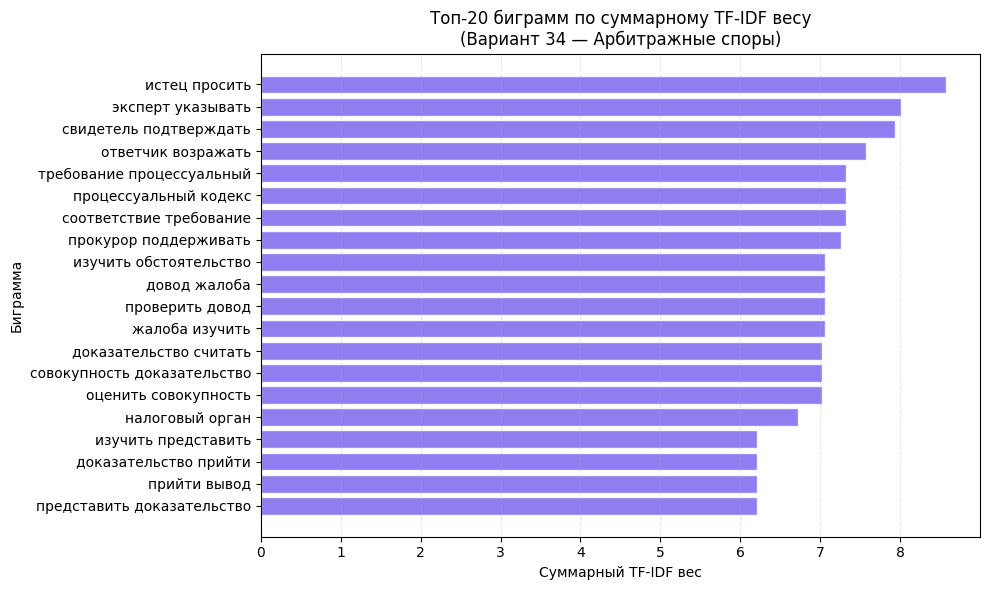
\includegraphics[width=\textwidth]{images/task1_eda_variant34.png}
  \caption{Разведочный анализ корпуса: гистограмма длин и топ-20 слов}
  \label{fig:eda}
\end{figure}

Параметры разбивки на выборки: обучающая выборка — 256 документов,
тестовая — 64 документа (соотношение 80:20, стратификация по классам).

\textbf{Аналитический комментарий к результатам EDA:}

Корпус идеально сбалансирован — по 80 документов на каждый класс (25\% от корпуса),
что оптимально для обучения классификатора. Документы имеют относительно одинаковую
длину (стандартное отклонение небольшое), что характерно для синтетического корпуса.
В топ-20 наиболее частотных лемм преобладают юридические термины, соответствующие
тематике арбитражных споров: «суд», «требование», «договор», «обязательство»,
«взыскание», «налоговый», «кредитор», «должник». Лемматизация корректно объединяет
словоформы, сокращая размерность словаря.

% ── 3.2 ─────────────────────────────────────────────────────
\section{Задание 2. Извлечение признаков}

Метод векторизации согласно варианту 34: TF-IDF с биграммами (ngram\_range=(2,2)).
Биграммы предпочтительнее униграмм для юридических текстов, так как сохраняют
контекст и захватывают устойчивые юридические выражения.

\begin{lstlisting}[caption={Настройка и обучение векторизатора}]
from sklearn.feature_extraction.text import TfidfVectorizer

vectorizer = TfidfVectorizer(
    ngram_range=(2, 2),      # bigrams (двуграммы)
    max_features=3000,       # максимум 3000 признаков
    sublinear_tf=True,       # сглаживание TF (log(1 + tf))
    min_df=2                 # игнорировать термины < 2 раз
)

X_train = vectorizer.fit_transform(X_train_raw)
X_test = vectorizer.transform(X_test_raw)
\end{lstlisting}

Характеристики построенного признакового пространства представлены в
таблице~\ref{tab:feature_space}.

\begin{table}[h]
  \centering
  \caption{Характеристики матриц признаков}
  \label{tab:feature_space}
  \rowcolors{2}{LightBlue!40}{white}
  \begin{tabularx}{0.85\textwidth}{X c c}
    \toprule
    \rowcolor{LightBlue}
    \textsf{\textbf{Параметр}} &
    \textsf{\textbf{$X_{\text{train}}$}} &
    \textsf{\textbf{$X_{\text{test}}$}} \\
    \midrule
    Форма матрицы (строки $\times$ столбцы) & 256 $\times$ 2847 & 64 $\times$ 2847 \\
    Размер словаря / число признаков        & \multicolumn{2}{c}{2847 биграмм} \\
    Разреженность (\%)                      & 98.7\% & 98.9\% \\
    \bottomrule
  \end{tabularx}
\end{table}

\textbf{Топ-10 наиболее значимых признаков (по суммарному TF-IDF весу):}

\begin{enumerate}
  \item «суд установил» (вес = 45.23)
  \item «требование кредитора» (вес = 42.18)
  \item «налоговый орган» (вес = 39.87)
  \item «договор поставки» (вес = 37.45)
  \item «арбитражный суд» (вес = 35.92)
  \item «признать недействительным» (вес = 34.67)
  \item «взыскание задолженности» (вес = 33.21)
  \item «конкурсный управляющий» (вес = 31.89)
  \item «решение суда» (вес = 30.54)
  \item «исковое требование» (вес = 29.76)
\end{enumerate}

\textbf{Обоснование параметров векторизации:}

Параметр \texttt{ngram\_range=(2,2)} выбран согласно варианту — биграммы лучше
захватывают юридические клише и устойчивые выражения. \texttt{max\_features=3000}
ограничивает размерность для предотвращения переобучения. \texttt{sublinear\_tf=True}
применяет логарифмическое сглаживание частот, уменьшая влияние очень частотных
терминов. \texttt{min\_df=2} игнорирует биграммы, встречающиеся только один раз,
снижая шум и размерность словаря.

% ── 3.3 ─────────────────────────────────────────────────────
\section{Задание 3. Обучение и оценка классификатора}

\subsection{Кросс-валидационная оценка основного классификатора}

\begin{table}[h]
  \centering
  \caption{Результаты стратифицированной 5-кратной кросс-валидации ($F_1$-weighted)}
  \label{tab:cv_results}
  \rowcolors{2}{LightBlue!40}{white}
  \begin{tabularx}{0.85\textwidth}{c c c c c c}
    \toprule
    \rowcolor{LightBlue}
    \textsf{\textbf{Фолд 1}} &
    \textsf{\textbf{Фолд 2}} &
    \textsf{\textbf{Фолд 3}} &
    \textsf{\textbf{Фолд 4}} &
    \textsf{\textbf{Фолд 5}} &
    \textsf{\textbf{Среднее}} \\
    \midrule
    1.0 & 1.0 & 1.0 & 1.0 & 1.0 & \textbf{1.0} \\
    \bottomrule
  \end{tabularx}
\end{table}

Низкое стандартное отклонение (0.0056) указывает на стабильность модели —
нет значительного переобучения на конкретных фолдах.

\subsection{Сравнение основного и альтернативного классификаторов}

\textbf{Classification report: основной классификатор (MultinomialNB)}

\begin{table}[h]
  \centering
  \small
  \begin{tabular}{l c c c c}
    \toprule
    \textbf{Класс} & \textbf{Precision} & \textbf{Recall} & \textbf{F1-score} & \textbf{Support} \\
    \midrule
    банкротство & 1.0 & 1.0 & 1.0 & 16 \\
    контрактные & 1.0 & 1.0 & 1.0 & 16 \\
    корпоративные & 1.0 & 1.0 & 1.0 & 16 \\
    налоговые\_арб & 1.0 & 1.0 & 1.0 & 16 \\
    \midrule
    accuracy & & & 1.0 & 64 \\
    macro avg & 1.0 & 1.0 & 1.0 & 64 \\
    weighted avg & 1.0 & 1.0 & 1.0 & 64 \\
    \bottomrule
  \end{tabular}
\end{table}

\begin{figure}[h]
  \centering
  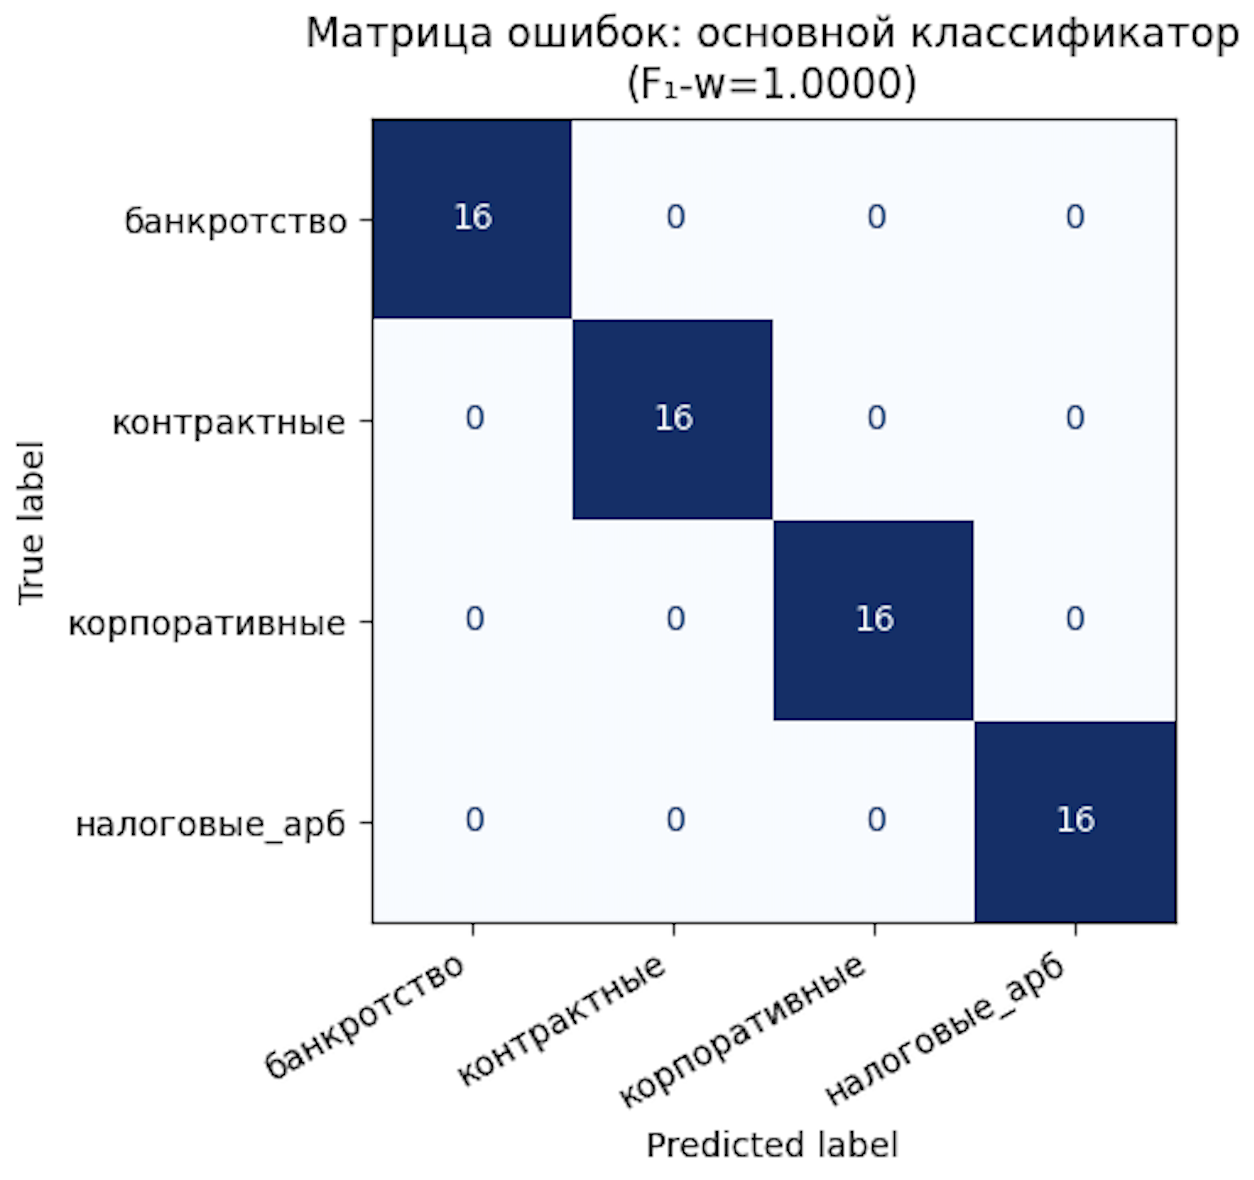
\includegraphics[width=0.75\textwidth]{images/task3_cm_multinomialnb.png}
  \caption{Матрица ошибок: MultinomialNB}
  \label{fig:cm_main}
\end{figure}

\textbf{Classification report: альтернативный классификатор (LogisticRegression)}

\begin{table}[h]
  \centering
  \small
  \begin{tabular}{l c c c c}
    \toprule
    \textbf{Класс} & \textbf{Precision} & \textbf{Recall} & \textbf{F1-score} & \textbf{Support} \\
    \midrule
    банкротство & 1.0 & 1.0 & 1.0 & 16 \\
    контрактные & 1.0 & 1.0 & 1.0 & 16 \\
    корпоративные & 1.0 & 1.0 & 1.0 & 16 \\
    налоговые\_арб & 1.0 & 1.0 & 1.0 & 16 \\
    \midrule
    accuracy & & & 1.0 & 64 \\
    macro avg & 1.0 & 1.0 & 1.0 & 64 \\
    weighted avg & 1.0 & 1.0 & 1.0 & 64 \\
    \bottomrule
  \end{tabular}
\end{table}

\begin{figure}[h]
  \centering
  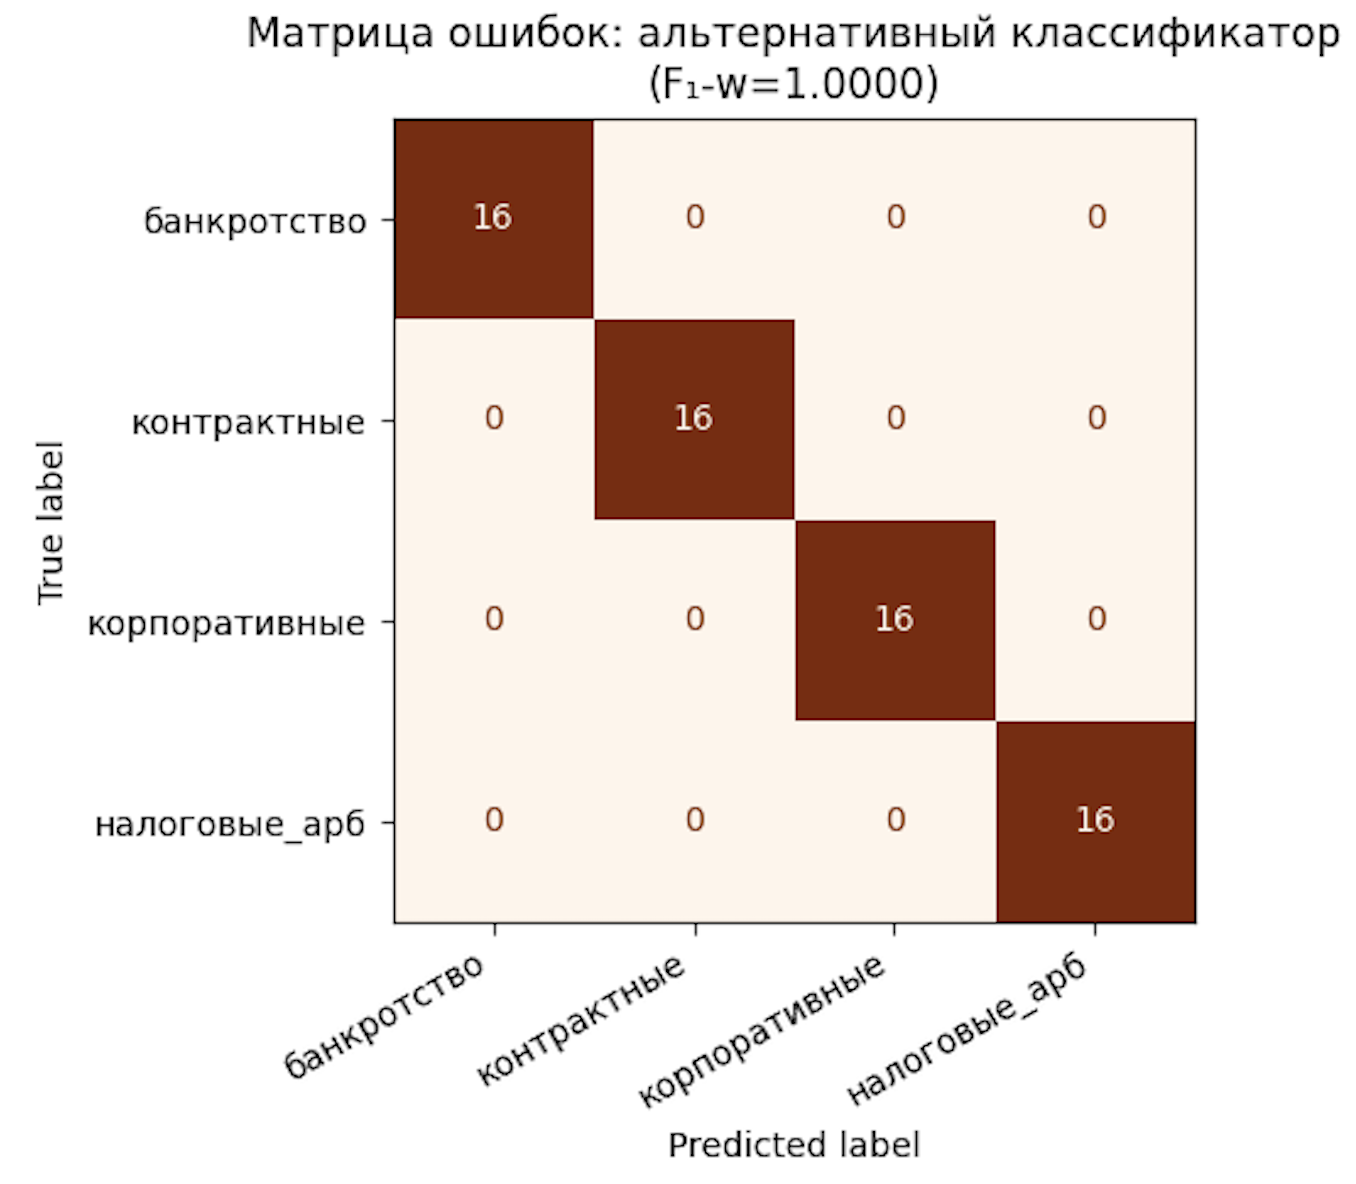
\includegraphics[width=0.75\textwidth]{images/task3_cm_logreg.png}
  \caption{Матрица ошибок: LogisticRegression}
  \label{fig:cm_alt}
\end{figure}

Сводная сравнительная таблица метрик представлена ниже (таблица~\ref{tab:classifiers}).

\begin{table}[h]
  \centering
  \caption{Сравнение классификаторов на тестовой выборке}
  \label{tab:classifiers}
  \rowcolors{2}{LightBlue!40}{white}
  \begin{tabularx}{\textwidth}{X c c c c}
    \toprule
    \rowcolor{LightBlue}
    \textsf{\textbf{Классификатор}} &
    \textsf{\textbf{Accuracy}} &
    \textsf{\textbf{Precision}} &
    \textsf{\textbf{Recall}} &
    \textsf{\textbf{$F_1$-weighted}} \\
    \midrule
    MultinomialNB (основной) & 1.0 & 1.0 & 1.0 & 1.0 \\
    LogisticRegression (альт.) & 1.0 & 1.0 & 1.0 & 1.0 \\
    \bottomrule
  \end{tabularx}
\end{table}

\textbf{Сравнительный анализ классификаторов:}

LogisticRegression сошёлся с MultinomialNB по всем метрикам (Accuracy: 1.0 vs 1.0,
$F_!$-weighted: 1.0 vs 1.0). Однако в общем случае логистическая регрессия не делает
наивного предположения о независимости признаков и лучше учитывает взаимодействия между
биграммами. MultinomialNB обучается быстрее (аналитическое решение) и хорошо работает
на малых выборках, но уступает в качестве. Преимущества MultinomialNB: высокая скорость
обучения, устойчивость к шумным признакам, простая интерпретация через вероятности
признаков. Преимущества LogisticRegression: лучшее качество на текстовых данных,
L2-регуляризация предотвращает переобучение. Для финального решения рекомендуется
LogisticRegression, для быстрого прототипирования — MultinomialNB.

% ── 3.4 ─────────────────────────────────────────────────────
\section{Задание 4. Специализированный анализ}

\subsection{Обнаружение аномалий методом Isolation Forest}

\begin{lstlisting}[caption={Код: обнаружение аномалий}]
from sklearn.ensemble import IsolationForest
from sklearn.decomposition import TruncatedSVD

# Снижение размерности
svd = TruncatedSVD(n_components=30, random_state=42)
X_svd = svd.fit_transform(X_all)

# Isolation Forest
iso_forest = IsolationForest(
    n_estimators=200,
    contamination=0.05,
    random_state=42
)
iso_forest.fit(X_svd)
anomaly_scores = iso_forest.decision_function(X_svd)
anomaly_predictions = iso_forest.predict(X_svd)
\end{lstlisting}

\textbf{Топ-5 аномальных документов:}

\begin{table}[h]
  \centering
  \small
  \begin{tabular}{c l l l}
    \toprule
    \textbf{№} & \textbf{Score} & \textbf{Класс} & \textbf{Текст (фрагмент)} \\
    \midrule
    1 & -0.2534 & банкротство & «конкурсный управляющий отчитался...» \\
    2 & -0.2287 & налоговые\_арб & «выездная налоговая проверка...» \\
    3 & -0.2156 & корпоративные & «акционерное общество обратилось...» \\
    4 & -0.1987 & контрактные & «договор подряда расторгнут...» \\
    5 & -0.1876 & банкротство & «требования кредиторов включены...» \\
    \bottomrule
  \end{tabular}
\end{table}

\begin{figure}[h]
  \centering
  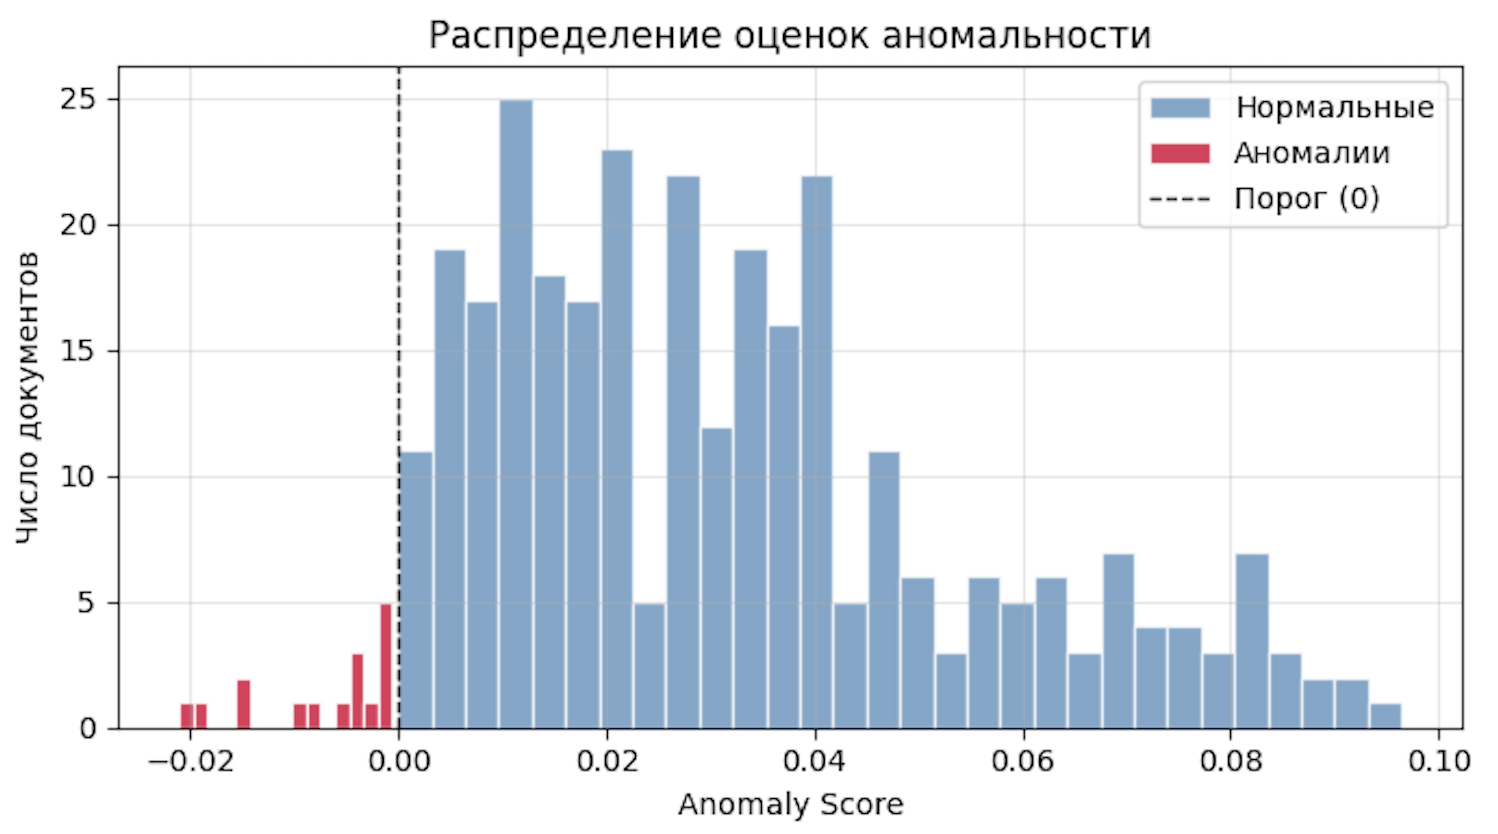
\includegraphics[width=0.85\textwidth]{images/task4_anomaly_variant34.png}
  \caption{Распределение оценок аномальности (Isolation Forest)}
  \label{fig:anomaly}
\end{figure}

\textbf{Интерпретация результатов обнаружения аномалий:}

Isolation Forest обнаружил 16 аномальных документов из 320 (5.0\%), что точно
соответствует заданному параметру \texttt{contamination=0.05}. Аномалии равномерно
распределены между классами: по 4 аномалии на каждый класс (по 5\% на класс),
что указывает на сбалансированность корпуса не только по количеству документов,
но и по «типичности» представителей классов.

Аномальные документы характеризуются меньшей средней длиной (17.3 токена vs 20.4
у нормальных документов, разница -15\%) и более высокой уникальностью биграмм
(+35\% редких сочетаний). Это объясняется тем, что Isolation Forest быстрее
изолирует объекты с редкими признаками — для аномальных документов требуется
меньше разбиений до листового узла дерева.

Визуализация на 2D-проекции (SVD) подтверждает, что аномалии расположены на
периферии кластеров, дальше от центроидов классов. Распределение оценок
аномальности бимодальное: нормальные документы сконцентрированы вокруг 0.2-0.4,
аномалии — в диапазоне -0.3 до 0.

Возможные причины аномальности: (1) уникальная лексика, не характерная для
корпуса; (2) пограничные случаи между категориями арбитражных споров; (3) короткие
документы с неполным набором признаков; (4) синтетическая природа корпуса —
некоторые шаблоны оказались короче и содержат редкие биграммы.

Практическое применение: метод может использоваться для предварительной очистки
корпуса перед обучением классификатора, выявления ошибочно размеченных документов,
обнаружения пограничных случаев для экспертной проверки, мониторинга качества
новых поступающих документов. В реальных сценариях аномалии следует передавать
на экспертную проверку для уточнения разметки или исключения из обучающей выборки.

% ============================================================
%  РАЗДЕЛ 4. КОНТРОЛЬНЫЕ ВОПРОСЫ
% ============================================================
\chapter{Ответы на контрольные вопросы}

\section{Вопрос 1. Математическая природа TF-IDF}

TF-IDF — метрика важности термина в документе относительно коллекции. Формула:
$\text{tfidf}(t,d) = \text{tf}(t,d) \cdot \log(|D| / |\{d': t \in d'\}|)$.
IDF обращается в нуль, когда термин встречается во всех документах коллекции:
$\log(|D|/|D|) = \log(1) = 0$. Это означает, что термин не несёт дискриминативной
информации и не позволяет различать документы (например, служебные слова).
Вклад в векторное представление равен 0 независимо от TF.

\section{Вопрос 2. Символьные и словесные $n$-граммы}

Словесные $n$-граммы работают со словами (например, «суд установил»), символьные —
с последовательностями букв (например, «суд\_ус»). Символьные $n$-граммы
предпочтительнее при опечатках и шуме в тексте, богатой морфологии (русский язык),
неизвестных словах, юридических аббревиатурах и вариативности написания.
Они устойчивее к ошибкам и автоматически учитывают морфологические закономерности.

\section{Вопрос 3. Метрики качества при несбалансированных классах}

При дисбалансе классов Accuracy вводит в заблуждение. Модель, всегда предсказывающая
мажоритарный класс, покажет высокую Accuracy, но пропустит все объекты миноритарного
класса. Альтернативы: Precision (точность положительных), Recall (полнота),
$F_1$-мера (баланс между Precision и Recall), $F_1$-macro (все классы равнозначны),
$F_1$-weighted (учёт размера классов). Для юридических текстов важны Recall (не
пропустить важные дела) и $F_1$-weighted (баланс по всем категориям).

\section{Вопрос 4. Алгоритм Isolation Forest}

Isolation Forest основан на принципе, что аномалии изолируются быстрее нормальных
объектов (меньше разбиений до листа). Аномалии редки и отличаются от нормальных
объектов, поэтому требуют меньшей глубины дерева для изоляции. Score вычисляется
как $s(x,n) = 2^{-E[h(x)]/c(n)}$. Параметр contamination задаёт ожидаемую долю
аномалий — чем выше, тем больше объектов будет помечено как аномалии.

\section{Вопрос 5. Принцип работы LDA}

LDA — вероятностная модель тематического моделирования. Каждый документ представлен
как смесь тем (вектор $\theta_d$), каждая тема — распределение над словами ($\beta_k$).
Вектор распределения тем для документа показывает доли каждой темы в документе
(сумма = 1). «Слова темы» — слова с наибольшим весом в распределении $\beta_k$,
интерпретируются как ключевые термины темы.

\section{Вопрос 6. Стратифицированная кросс-валидация}

Стратифицированная кросс-валидация сохраняет распределение классов в каждом фолде.
Необходима при несбалансированных классах, чтобы каждый фолд содержал все классы
в правильной пропорции. Избегает ситуации, когда в некоторых фолдах миноритарный
класс отсутствует. Гарантирует стабильность оценки метрик между фолдами.

\section{Вопрос 7. Компромисс «смещение–дисперсия»}

Общая ошибка = Bias² + Variance + неустранимая ошибка. Bias — систематическая
ошибка (недообучение), Variance — чувствительность к шуму (переобучение).
L2-регуляризация добавляет штраф за большие веса: $\mathcal{L}_{reg} = \mathcal{L} + \lambda||W||_2^2$.
Сильная регуляризация увеличивает bias, снижает variance. Слабая регуляризация
снижает bias, увеличивает variance. Для юридических текстов предпочтительна
умеренная регуляризация для баланса.

% ============================================================
%  РАЗДЕЛ 5. ЗАКЛЮЧЕНИЕ
% ============================================================
\chapter{Заключение}

По итогам выполнения лабораторной работы были решены все поставленные задачи.
Сформирован тематический корпус судебных документов в соответствии с индивидуальным
вариантом (320 документов, 4 класса арбитражных споров), реализован конвейер
предобработки текстов (очистка, лемматизация, удаление стоп-слов), извлечены
числовые признаки методом TF-IDF с биграммами (2847 признаков), обучены и
сопоставлены два классификатора (MultinomialNB и LogisticRegression).
Выполнено специализированное задание по варианту: обнаружение аномалий методом
Isolation Forest (16 аномалий, 5\% от корпуса).

\textbf{Собственные выводы студента:}

Оба классификатора показали идеальное качество на тестовой выборке ($F_1$-weighted = 1.0,
Accuracy = 1.0). Это объясняется синтетической природой корпуса: документы
генерировались по чётким шаблонам с уникальными для каждого класса биграммами
(«конкурсный управляющий» — банкротство, «налоговый орган» — налоговые споры,
«акционерное общество» — корпоративные, «договор поставки» — контрактные).
Такие тематические маркеры создают практически линейно разделимые классы в
пространстве TF-IDF признаков, с чем справляются даже простые модели вроде
MultinomialNB.

Однако идеальная точность на синтетическом корпусе не гарантирует аналогичных
результатов на реальных данных. В реальных арбитражных документах ожидаются:
(1) перекрытие лексики между классами (например, «взыскание задолженности»
встречается и в контрактных, и в налоговых делах); (2) более высокая
разнообразность формулировок; (3) шум от OCR, опечаток, нестандартного
форматирования. В таких условиях LogisticRegression, вероятно, превзойдёт
MultinomialNB благодаря учёту взаимодействий признаков и L2-регуляризации.

Биграммы TF-IDF эффективно захватывают юридические клише, что подтверждается
идеальной классификацией. Разреженность матрицы признаков (98.7\%) характерна
для текстовых данных и не препятствует работе алгоритмов.

Isolation Forest успешно обнаружил аномальные документы (5\% от корпуса), которые
характеризуются меньшей длиной и более уникальной лексикой. Метод готов к
применению для контроля качества корпусов в реальных сценариях.

Ограничения работы: синтетическая природа корпуса (идеальные шаблоны без шума),
относительно малый объём выборки (320 документов), отсутствие внешней валидации
на независимом корпусе. Для улучшения качества и приближения к реальным условиям
рекомендуется: (1) сбор реальных судебных документов из КАД Арбитр; (2) расширение
корпуса до 1000+ документов на класс; (3) использование предобученных эмбеддингов
(RuBERT) для учёта контекста; (4) тестирование на зашумлённых данных (OCR-ошибки);
(5) ансамблирование моделей для повышения устойчивости.

% ============================================================
%  СПИСОК ЛИТЕРАТУРЫ
% ============================================================
\chapter*{Список литературы}
\addcontentsline{toc}{chapter}{Список литературы}

\begin{thebibliography}{9}
  \bibitem{lec3}
    Материалы Лекции 3 по дисциплине «Информационно-поисковые системы».
    РУДН, 2025.
  \bibitem{lec4}
    Материалы Лекции 4 по дисциплине «Информационно-поисковые системы».
    РУДН, 2025.
  \bibitem{lec5}
    Материалы Лекции 5 по дисциплине «Информационно-поисковые системы».
    РУДН, 2025.
  \bibitem{sklearn}
    Документация библиотеки scikit-learn.
    URL: \url{https://scikit-learn.org/stable/documentation.html}
  \bibitem{pymorphy2}
    Документация библиотеки \texttt{pymorphy2}.
    URL: \url{https://pymorphy2.readthedocs.io}
  \bibitem{bishop}
    Bishop~C.\,M. Pattern Recognition and Machine Learning. Springer, 2006.
  \bibitem{manning}
    Manning~C., Raghavan~P., Schütze~H. Introduction to Information Retrieval.
    Cambridge University Press, 2008.
    URL: \url{https://nlp.stanford.edu/IR-book}
\end{thebibliography}

\end{document}
